\documentclass[11pt,a4paper]{report}
\usepackage[utf8]{inputenc}
\usepackage{ucs}
%\usepackage{fullpage}
\usepackage[english]{babel}
\usepackage{verbatim}
\usepackage{amsmath}
\usepackage{amsfonts}
\usepackage{amssymb}
\usepackage[pdftex]{graphicx}
\usepackage{makeidx}
\makeindex
\usepackage{array}
%\usepackage{multirow}
\usepackage{color}
%\usepackage{moreverb}
\usepackage{listings} 
\definecolor{colKeys}{rgb}{0,0,1} 
\definecolor{colIdentifier}{rgb}{0,0,0} 
\definecolor{colComments}{rgb}{0,0.5,1} 
\definecolor{colString}{rgb}{0.6,0.1,0.1} 
\lstset{ 
language=java,
basicstyle=\ttfamily\small, % 
identifierstyle=\color{colIdentifier}, % 
keywordstyle=\color{colKeys}, % 
stringstyle=\color{colString}, % 
commentstyle=\color{colComments}, 
columns=flexible,
tabsize=5,
%frame=single,
frame=shadowbox,
rulesepcolor=\color[gray]{0.5},
extendedchars=true,
showspaces=false,
showstringspaces=false,
numbers=left,
numberstyle=\tiny,
breaklines=true,
%backgroundcolor=\color{hellgelb},
captionpos=b,%
%morekeywords={AND,ASC,avg,CHECK,COMMIT,count,DECODE,DESC,DISTINCT,%
%GROUP,IN,LIKE,NUMBER,ROLLBACK,SUBSTR,sum,VARCHAR2,iif},%
} 

\usepackage{url} 
\usepackage{fancyhdr}
\usepackage{caption}
\pagestyle{fancy}
\renewcommand{\headrulewidth}{0pt}
\fancyhead{}
\fancyfoot{}


\begin{document}

%%%%%%%%%%%%%%%%%%%%
% MAIN PAGE %
%%%%%%%%%%%%%%%%%%%%
\begin{titlepage}

	%\vspace*{2cm}


	\begin{flushleft}
		 \includegraphics*[width=4cm]{logo.jpg} \\
		 \textsl{12, rue de la Houssinière}\\
		 \textit{44322 Nantes}
		\hrulefill
	\end{flushleft}


	\vspace{2cm}


	\begin{flushleft}

		{\fontfamily{ppl}\fontseries{b}\fontsize{1.4cm}{1.65cm}\selectfont ObiGO  } 	 \\ 
	
		\vspace{1cm}
	
		{\Large Technical Documentation}\\
	
		\vspace{1cm}
		Adrien Guille \\
		Vincent Ferreira \\
		\textit{2009-2010}
	
	\end{flushleft}

	\vspace{2cm}

	\begin{flushleft}
	 	\textsc{Master 1 - ALMA}\\	
	 	\hrulefill
	\end{flushleft}


\end{titlepage}
% \hspace{\stretch{1}}

%%%%%%%%%%%%%%%%%%%%
% TABLE OF CONTENTS %
%%%%%%%%%%%%%%%%%%%%
\tableofcontents

%%%%%%%%%%%%%%%%%%%%
% DOC %
%%%%%%%%%%%%%%%%%%%%
\chapter*{Heuristic}
\addcontentsline{toc}{chapter}{Heuristic}


The heuristic is used to describe the process by which the computer can solve the complex problem of evaluating a state of game.
Its purpose is to calculate a value for a given game state. The more the game state tends towards a conclusive situation for the current player, the more the value must be high.\\

A situation will be conclusive when the current player takes the advantage over his opponent.
Overall a situation is considered conclusive if the player takes more stones than it loses.\\

The heuristic is applied after the first two moves made by the computer, which are determined randomly.\\
\newpage 

\section*{Rating Scale}
\addcontentsline{toc}{section}{Rating scale}

For a general consistency of the calculated scores, it is essential to establish a standard scale. Our scale consists of eight levels:\\

\begin{tabular}{|c|c|c|c|c|c|c|c|}
\hline EXCELLENT & VERYGOOD & GOOD & PLUS & MINUS & BAD & VERYBAD & AWFUL \\ 
\hline 750 & 500 & 250 & 100 & -100 & -250 & -500 & -750 \\ 
\hline 
\end{tabular} \\

\begin{figure}[h]
\centering
\includegraphics[width=0.75\textwidth]{Rating_Scale.png}
\caption{Graphical representation of the rating scale}
\label{rating_scale}
\end{figure}

\section*{Components}
\addcontentsline{toc}{section}{Components}


The overall heuristic uses several internal components. The order of consultation of the components is essential. We must examine the components in an order corresponding to their importance in making a final decision.\\


All components take the goban to test and the color of the current player as parameters. A component can return three values: -1, 0 and 1. 
-1 means that the component is checked for the enemy player, 0 that is not validated and 1 that it is validated for the current player.\\

The components are:\\

\textbf{deltaCaught}: differential between the amount of stones caught by the current player and the opponent.\\

\textbf{hasCaught}: Returns 1 if this move leads to a wall of pawns by the player, -1 if the player is taken, 0 if no pieces are taken.\\

\textbf{commonBorder}: Returns 1 if the current player is in contact with enemy territory, -1 if the opponent is in contact with the current player.\\

\textbf{underNGroups}: This component is parameterized by an integer n. Returns 1 if the current player maintains less than n groups, while forcing the opponent to exceed n. The score are inversed if the component is applied to a move made by the opponent.\\



We articulate our assessment around these components. The note is initialized to 0, then we follow the order of consultation until a component meets and achieves a score different from 0. It therefore stops at the first decisive response of a component (ie a response -1 or 1).
The assessment takes the value associated with the component level, with a positive or negative sign depending of the response of the component.\\

\bigskip

For example, if the component isCaught returns -1, a score of -750 is affected, corresponding to VERYBAD. By cons, if it meets 1, a score of 750, VERYGOOD, is returned. If isCaught returns 0, then we ask the next component.\\



Here is an activity diagram representing the inter-component articulation :

\begin{figure}[h]
\centering
\includegraphics[width=1\textwidth]{activity_diagram.png}
\caption{Activity diagram of the evaluation}
\label{activity_diagram}
\end{figure}

\chapter*{Implementation}
\addcontentsline{toc}{chapter}{Implementation}

\section*{Program Architecture}
\addcontentsline{toc}{section}{Program Architecture}

\subsection*{Package Diagram}
\addcontentsline{toc}{section}{Package Architecture}

\begin{center}
	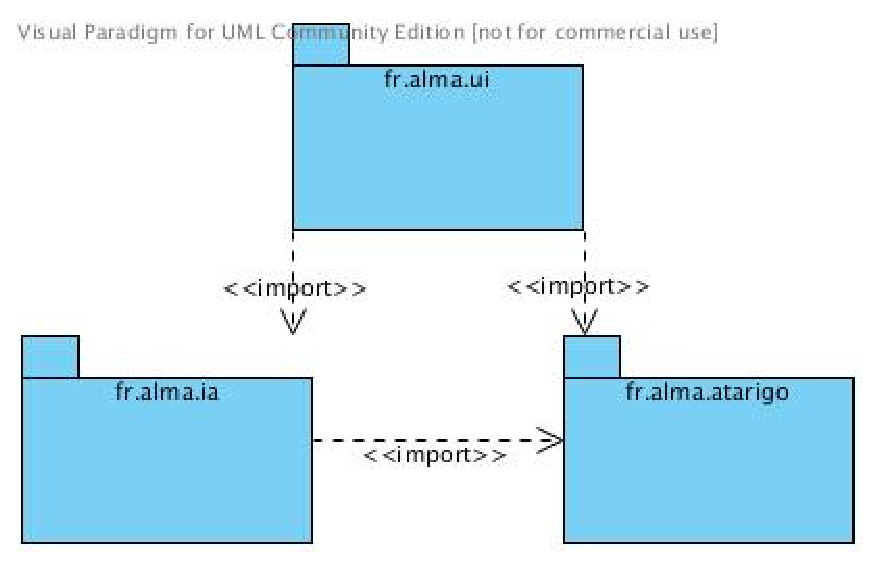
\includegraphics[scale=0.70]{package_diag}
	\captionof{figure}{Package diagram of Obigo}
\end{center}

    Our program is organized in three packages. "fr.alma.atarigo" which represents the rules and mechanisms of atarigo then, the package "fr.alma.ia" which is responsible for calculations of artificial intelligence and finally, the package "fr.alma.ui" representing the user interface which communicate with the game.

\subsection*{Class Diagram}
\addcontentsline{toc}{subsection}{Class Diagram}


\subsubsection*{AtariGo}
\addcontentsline{toc}{subsubsection}{AtariGo}


\begin{center}
	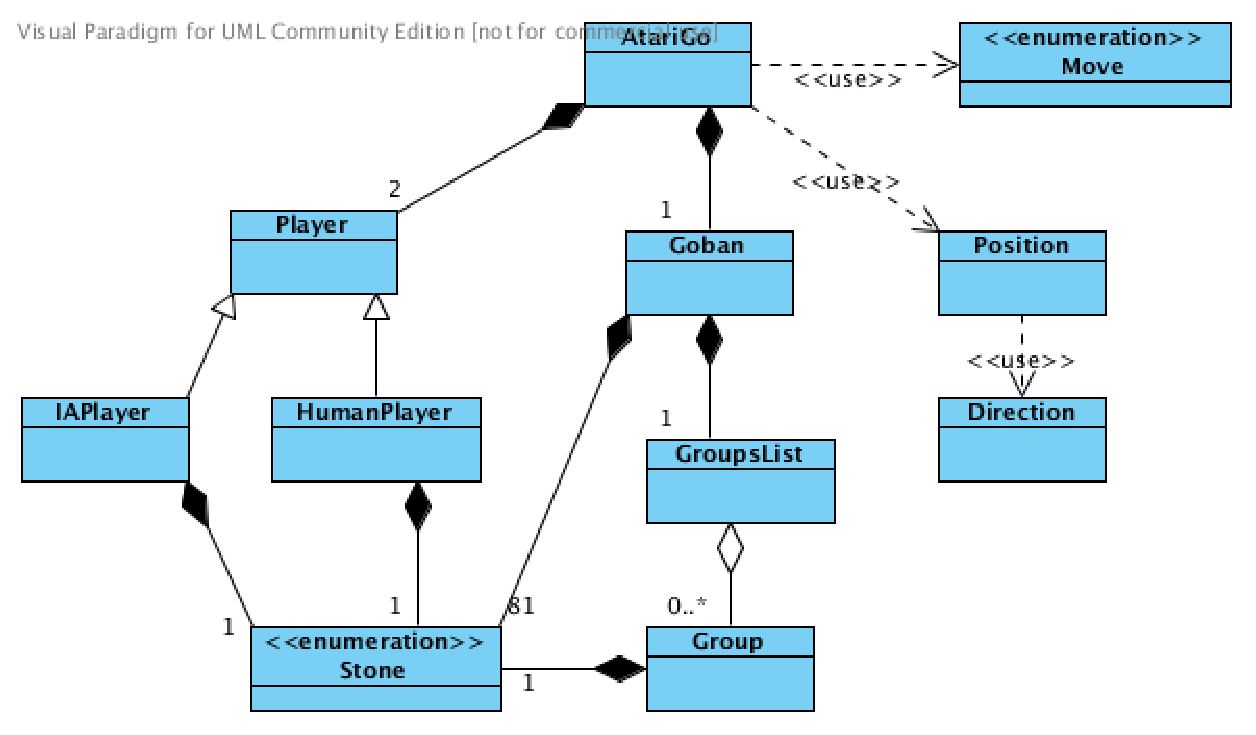
\includegraphics[scale=0.70]{class_diag}
	\captionof{figure}{Class diagram of AtariGo}
\end{center}

    Here is a view of classes interactions in the Atarigo Package. We can see that the class Atarigo is at the center of the package.It has the method "playMovie" that does all the mechanisms created by the move of a pawn.
    When calling this method, there put a stone on the board and return the type of move. This type is defined in the enumerated class Move. If INVALID, the move is not playable, if WIN at least once captured a pawn and, finally, if it is NEUTRAL, the move is playable without causing catch.
The algorithm returning these statements makes all the possible checks on the position played and especially with the method called by the class writeCell Goban.

\subsubsection*{Goban}
\addcontentsline{toc}{subsubsection}{Goban}


	The class contains the board game and owns several methods for the analysis of Goban. It contains a square matrix of the type listed STONE. This type is either BLACK to represent a box containing a black stone, WHITE for a white stone or EMPTY for an empty square. As can be seen in the class diagram, class STONE is also used to set the color played by a player or the color of a group of stones.\\

Position and Direction classes are classes facilitating access to positions of Goban.\\

    The class also has an instance of GroupsList. This class represents a list of all groups of stones from the game. A group is a set of stones of the same color connected to another one vertically and horizontally. It is necessary to store the list of groups to keep a clear view of the state.

\chapter*{Optimizing AI}
\addcontentsline{toc}{chapter}{Optimizing AI}
 

For artificial intelligence playing a game, time is critical. With infinite time, it is shown that the MinMax method (based on a good heuristic) will always find the ideal configuration of play. But the time allowed for reflection during a game is rarely infinite. Therefore, the more the computer can process data faster, the more it will deepen its reflection (and be stronger). \\

For this, two parameters are taken into account: The computational complexity mentioned above, but also the complexity in memory. \\

From the perspective of memory, the main issue is the storage representation of a Goban. Several solutions are available to us: \\
     
 \begin{itemize}
\item    Use a square matrix modeling entire goban (a grid of color and empty squares). 
\item    Use a list of played stones only (couples position / color). 
\end{itemize}
\bigskip

Both solutions have each an argument in their favor and one against them. \\

Indeed, the matrix provides a constant time access, access is O(1). For cons, the Goban still occupies the same memory space whether it's empty or full (81 times the size of an integer), and demands a contiguous memory space . It is therefore an important loss. \\

The list of played stones occupies minimal memory space, and does not require to have a contiguous space. By cons, data access is done this time  in O(n). 
\bigskip



In response to his arguments, a question arises: what should we focus on? The access time or the memory space? 

We have chosen to represent the Goban by a matrix. In effect, this allows us to have excellent speed, and as we use the alphabet, the memory savings permitted by the pruning-induced memory loss offsets not matrixes (This choice is even more reasoned that Today machines have huge amounts of memory, for example, a macbook has at least 4GB).

\end{document} 
